\subsection[Scenariusz - Pharming (Jakub Wyka)]{Scenariusz - Pharming}
\label{sce:phar}
Zatruwanie DNS to metoda ataku polegająca zmianie lokalnego rekordu DNS, który
fałszywie przypisuje nazwę domeny do adresu IP.  
Zadaniem tego ataku jest przekierowanie użytkownika na inną stronę niż ta,
 którą faktycznie chciał otworzyć. Często witryna podszywająca się wygląda 
 tak samo, przez co użytkownik nie jest świadomy ataku. Podszywanie to jest 
 nazywane phishingiem. W ten sposób użytkownik logując się do serwisu dostarcza 
 wrażliwe dane osobom przeprowadzającym atak. Połączenie DNS spoofingu z 
 zaawansowanym phishingiem nazywane jest pharmingiem.
 \subsubsection[Aktorzy]{Aktorzy}
 \begin{itemize}
     \item 	Pentester
     \item 	Serwer sterujący
     \item 	Testowany system
     \item   Urządzenie wykonujące
 \end{itemize}
 \subsubsection[Założenia początkowe]{Założenia początkowe}
Urządzenie wykonujące powinno być podłączone do internetu za pomocą sieci wi-fi oraz połączone
z testowanym komputerem za pomocą przewodu usb - micro usb. Ważne jest również aby było podłączone
do serwera, który zarządza wykonywaniem testów.
Ważne jest również aby osoba wykonująca test - pentester, była zalogowana do serwera.
 \subsubsection[Przebieg testu]{Przebieg testu}
Serwer sterujący służy do wydawania poleceń przez pentestera. 
Wybiera on, za pomocą którego z dostępnych urządzeń testujących 
ma zostać przeprowadzony test. Następnie wybiera rodzaj testu. W tym 
przypadku będzie to pharming. Serwer udostępni możliwość określenia
 konkretnych parametrów testu. Dla tego typu testu będzie to rekord DNS,
  który określi pod jaką domenę chcemy się podszyć oraz ip strony podszywającej. 
  Serwer przesyła te dane do urządzenia wykonującego, które na tej podstawie uruchamia 
  skrypt, który jest odpowiedzialny za przeprowadzenie testu. Do serwera odsyłany
jest raport z wynikiem testu. 
\begin{figure}[H]
    \centering
    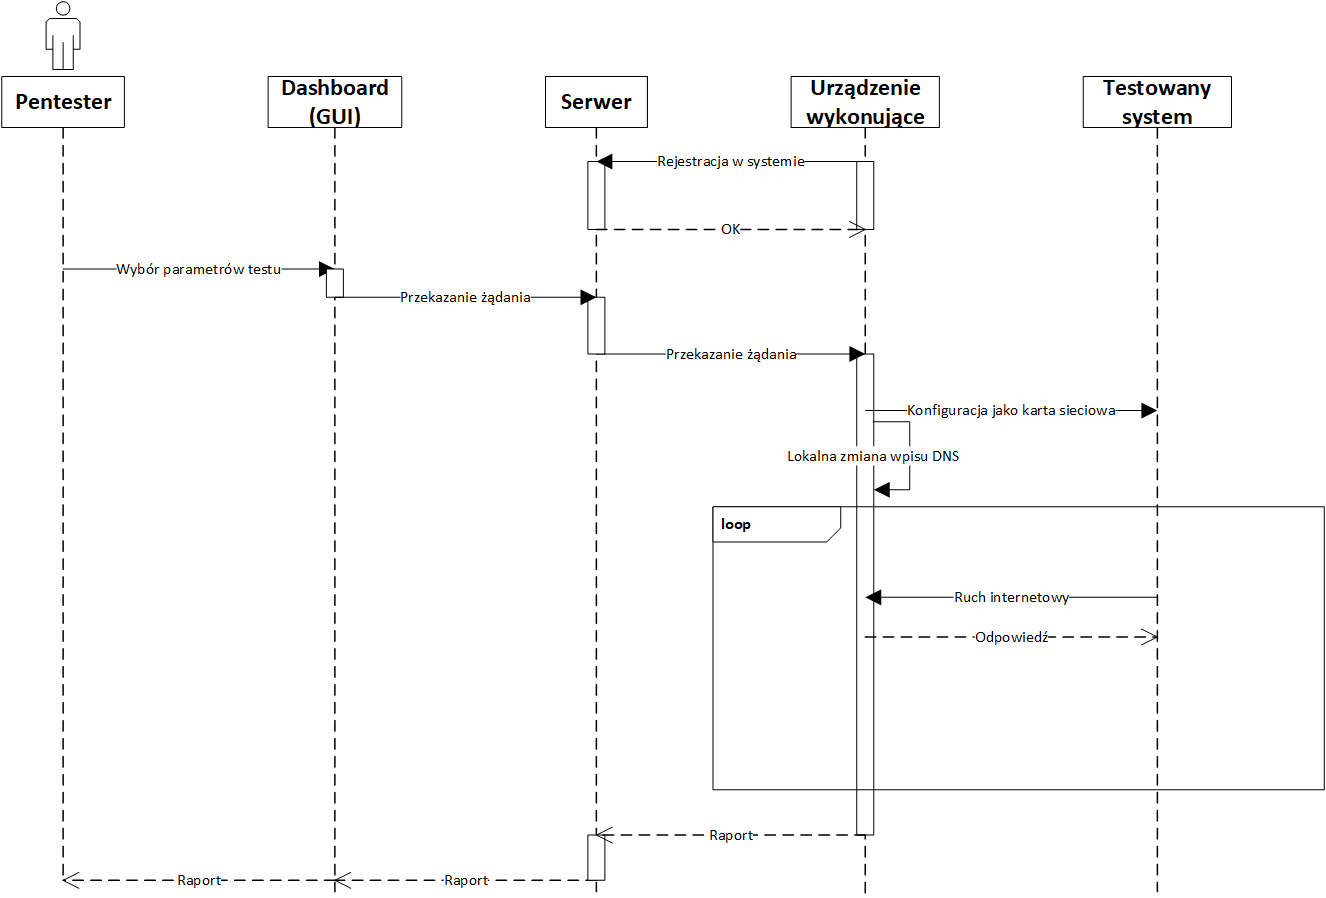
\includegraphics[width=\textwidth]{interJW}
    \caption{Diagram interakcji dla scenariusza testowego "Pharming"}
    \label{fig:pharming1}    
\end{figure}
\begin{figure}[H]
    \centering
    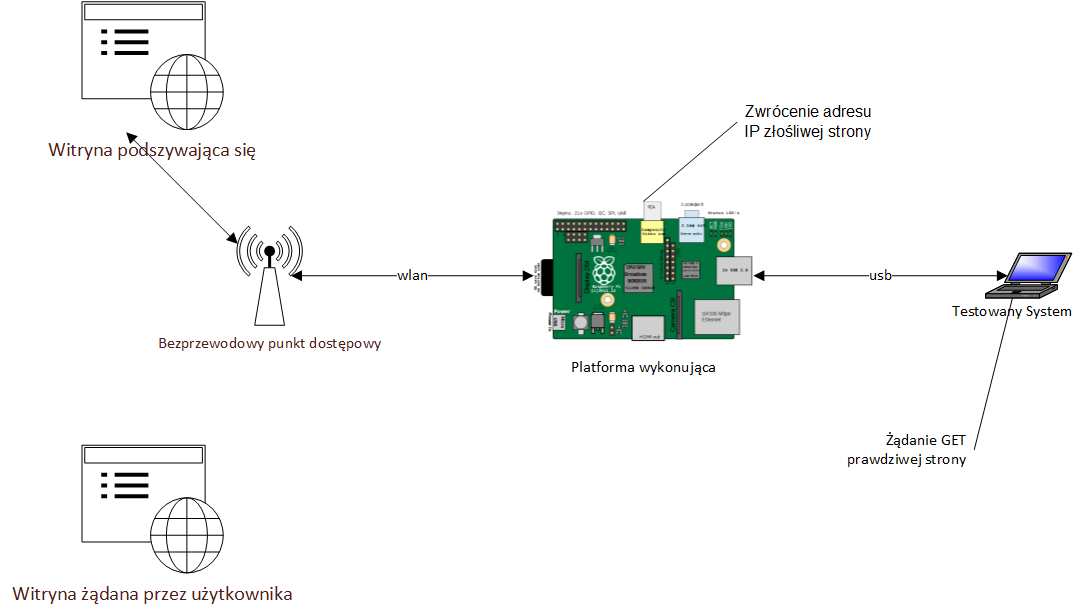
\includegraphics[width=\textwidth]{ks2}
    \caption{Diagram przedstawiający zasadę działania testu bezpieczenśtwa "Pharming"}
    \label{fig:pharming2}    
\end{figure}

\subsubsection[Mozliwosc wykrycia]{Możliwość wykrycia }
\label{subsec:wykrpharming}
Phishing jest metodą oszustwa opartą na inżynieri społecznej.
Ten scenariusz testowy ma więc na celu przetestowanie zachowania człowieka, który jest użytkownikiem systemu.
Wynika to z faktu, że jego głównym celem jest przekierowanie go na podszywającą się witrynę i
 wydobycie od niego wrażliwych danych. Należy więc zauważyć, że podmiana rekordu dns jest jedynie środkiem
 do udanego przeprowadzenia symulacji ataku phishingowego.
 Alternatywnym sposobem mogłoby być rozesłanie wiadomości drogą elektroniczą ze złośliwym hiperłączem, jednak
 atutem rozwiązania korzystającego z urządzenia USB jest możliwość przetestowania świadomości użytkowników
 na temat niebezpieczeństw jakie niosą nieznane urządzenia podłączane do systemu.
Możliwość wykrycia złośliwego urządzenia w konfiguracji karty sieciowej została opisana
 w sekcji~\ref{subsec:wykrywalnoscJW},
więc w tym rozdziale zostanie ona przeanalizowana dla szczególnego przypadku jakim jest
test bezpieczeństwa pod kątem ataku "phishing".
Kluczowe w dbaniu o autentyczność witryny są certyfikaty SSL. Istotny jest również ich rodzaj, gdyż wyróżniamy~\cite{ssltypes}:
\begin{itemize}
    \item Domain Validation SSL certificates (DV) 
    \subitem Jest to najszybszy i najprostszy sposób uzyskania certyfikatu SSL. Weryfikowana jest tylko domena.
    \item Organization Validation (OV)
    \subitem Na potrzeby uzyskania tego certyfikatu weryfikowana jest nie tylko domena, a także organizacja wnioskująca o jego uzyskanie. 
    Dzięki temu certyfikat zapewnia wyższy poziom bezpieczeństwa od certyfikatu SSL DV.
    \item Extended Validation SSL certificates (EV)
    \subitem Certyfikat zapewnia najwyższy poziom zaufania i bezpieczeństwa, dzięki długiemu procesowi
    weryfikacji. Trwa on nawet kilka tygodni, przez co jest kosztowny.
    Jednak najważniejsze jest to, że proces dokładnego sprawdzenia organizacji wnioskującej 
    o certyfikat zapewnia ochronę przed atakami typu phishing.      
\end{itemize}
Podsumowując, samo posiadanie certyfikatu ssl może nie być  wystarczające aby 
jednoznacznie potwierdzić bezpieczeństwo witryny. 
Użytkownicy powinni zwracać uwagę na obecność Extended Validation SSL certificate, a jego brak
 powinien wzbudzać czujność internauty lub nawet być powodem do opuszczenia danej strony.


\begin{figure}[H]
        \centering
        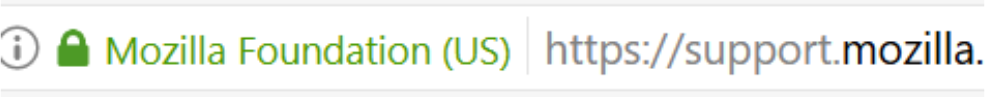
\includegraphics[width=\textwidth]{ev}
        \caption{Przykład wizualizacji posiadania certyfikatu EV przez daną witrynę, zaczerpnięty z~\cite[]{sslev}}
        \label{fig:ev}
    \end{figure}